\section{Избранные фотографии из личного фотоархива М. П.~Шубича}

\begin{figure}[h]
\includegraphics[width=\textwidth,center]{private/armiyaPatrul_1955}
\caption{Патрули по˚городку. Школа сержантского состава. М.\,П.~Шубич крайний справа. Г.~Киев, 1955~год.}
\label{fig:armiyaPatrul_1955}
\end{figure}

\begin{figure}[h]
\includegraphics[height=.8\textwidth, width=\textheight, keepaspectratio, angle=90, center]{private/armiyaKross10km_1955}
\caption{После˚10\,км кросса. Школа сержантского состава (первый год службы). М.\,П.~Шубич четвёртый военнослужащий слева. Г.~Киев, 1955~год.}
\label{fig:armiyaKross10km_1955}
\end{figure}


\begin{figure}[h]
\includegraphics[height=.8\textwidth, width=\textheight, keepaspectratio, angle=90, center]{private/nagradaShubichBoevoeZnamyaOborot}
\caption{Поощрение М.\,П.~Шубича фотографией с˚боевым знаменем части. 1958~год.}
\label{fig:nagradaShubichBoevoeZnamyaOborot}
\end{figure}

\begin{figure}[h]
\includegraphics[width=\textwidth]{private/rectorKostirev}
\caption{Леонид Семёнович Костырев. Бывший ректор МИИЗа, заведующий кафедрой экономики.}
\label{fig:rectorKostirev}
\end{figure}


\begin{figure}[h]
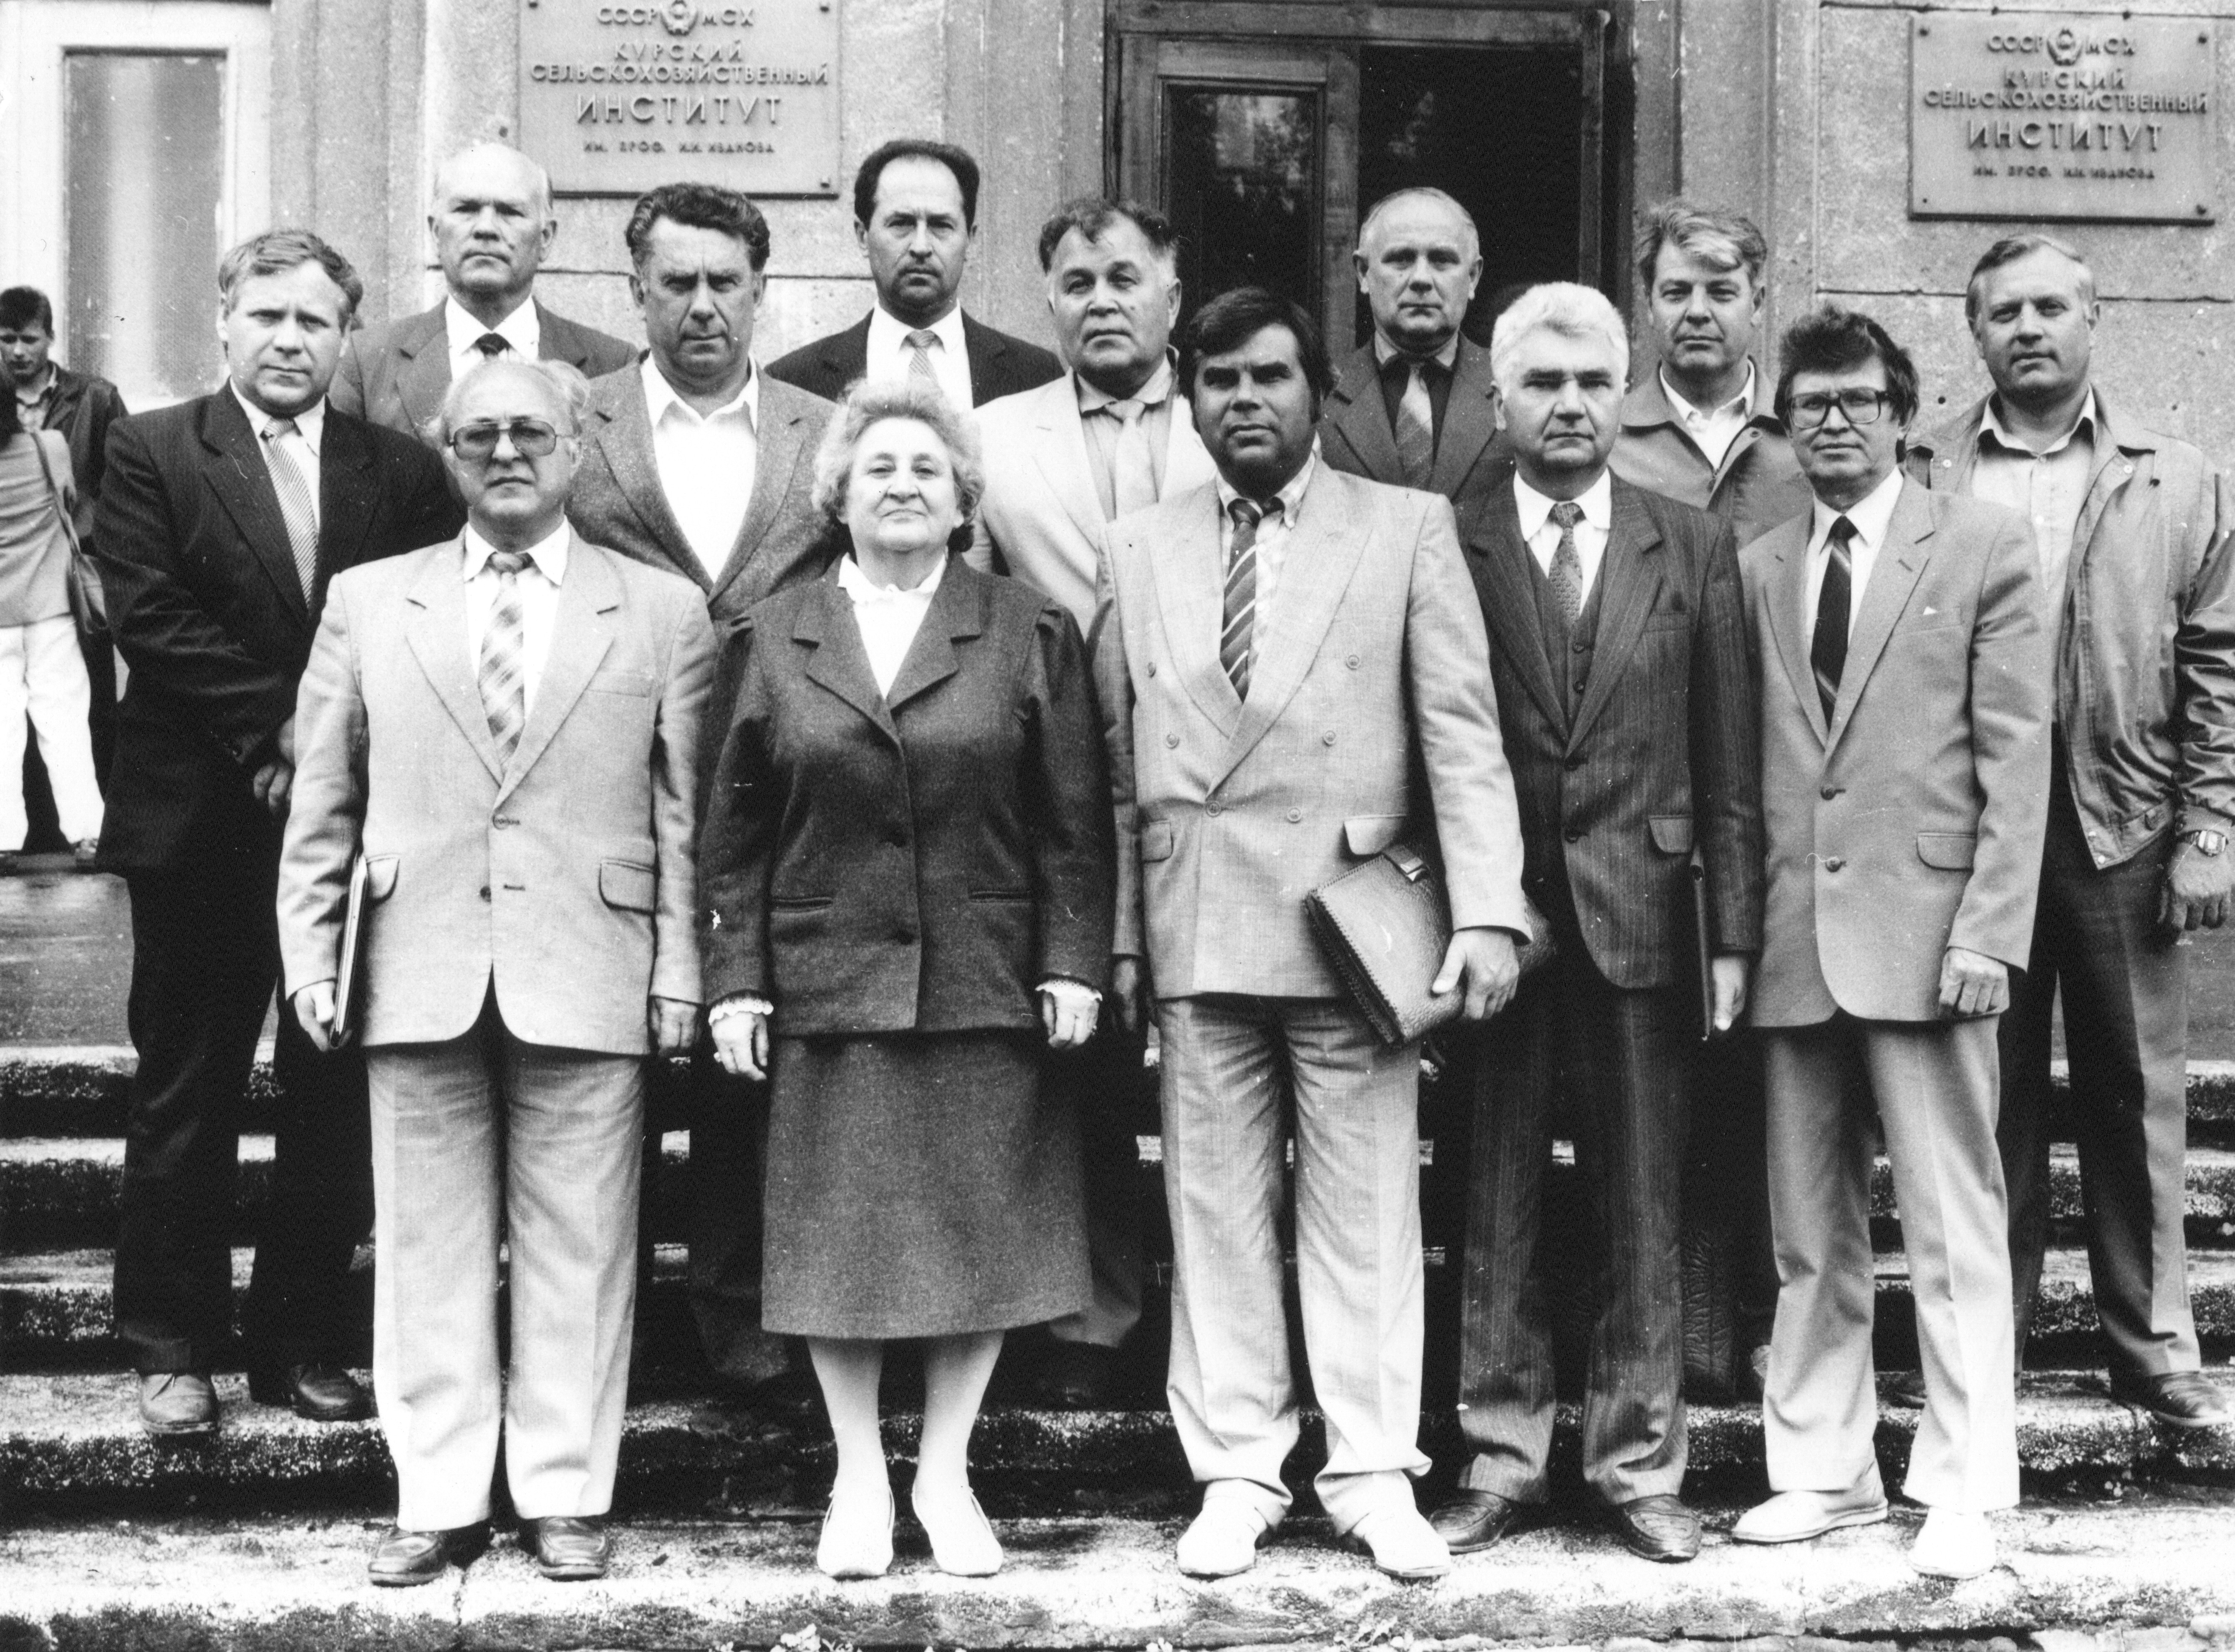
\includegraphics[height=.9\textwidth, width=\textheight, keepaspectratio, angle=90, center]{private/UchebMetodichSovet}
\caption{Учебно\-/методический совет по˚заочному образованию Главного управления. Семинар 14\==18.06.1993, Курск-СХИ. М.\,П.~Шубич второй справа в˚1\=/ом ряду.}
\label{fig:UchebMetodichSovet}
\end{figure}

\begin{figure}[h]
\includegraphics[height=.9\textwidth, width=\textheight, keepaspectratio, angle=90, center]{private/KomissiyaDiplom_1982}
\caption{Комиссия по˚защите дипломных проектов. М.\,П.~Шубич второй справа. 1982~год.}
\label{fig:KomissiyaDiplom_1982}
\end{figure}

\begin{figure}[h]
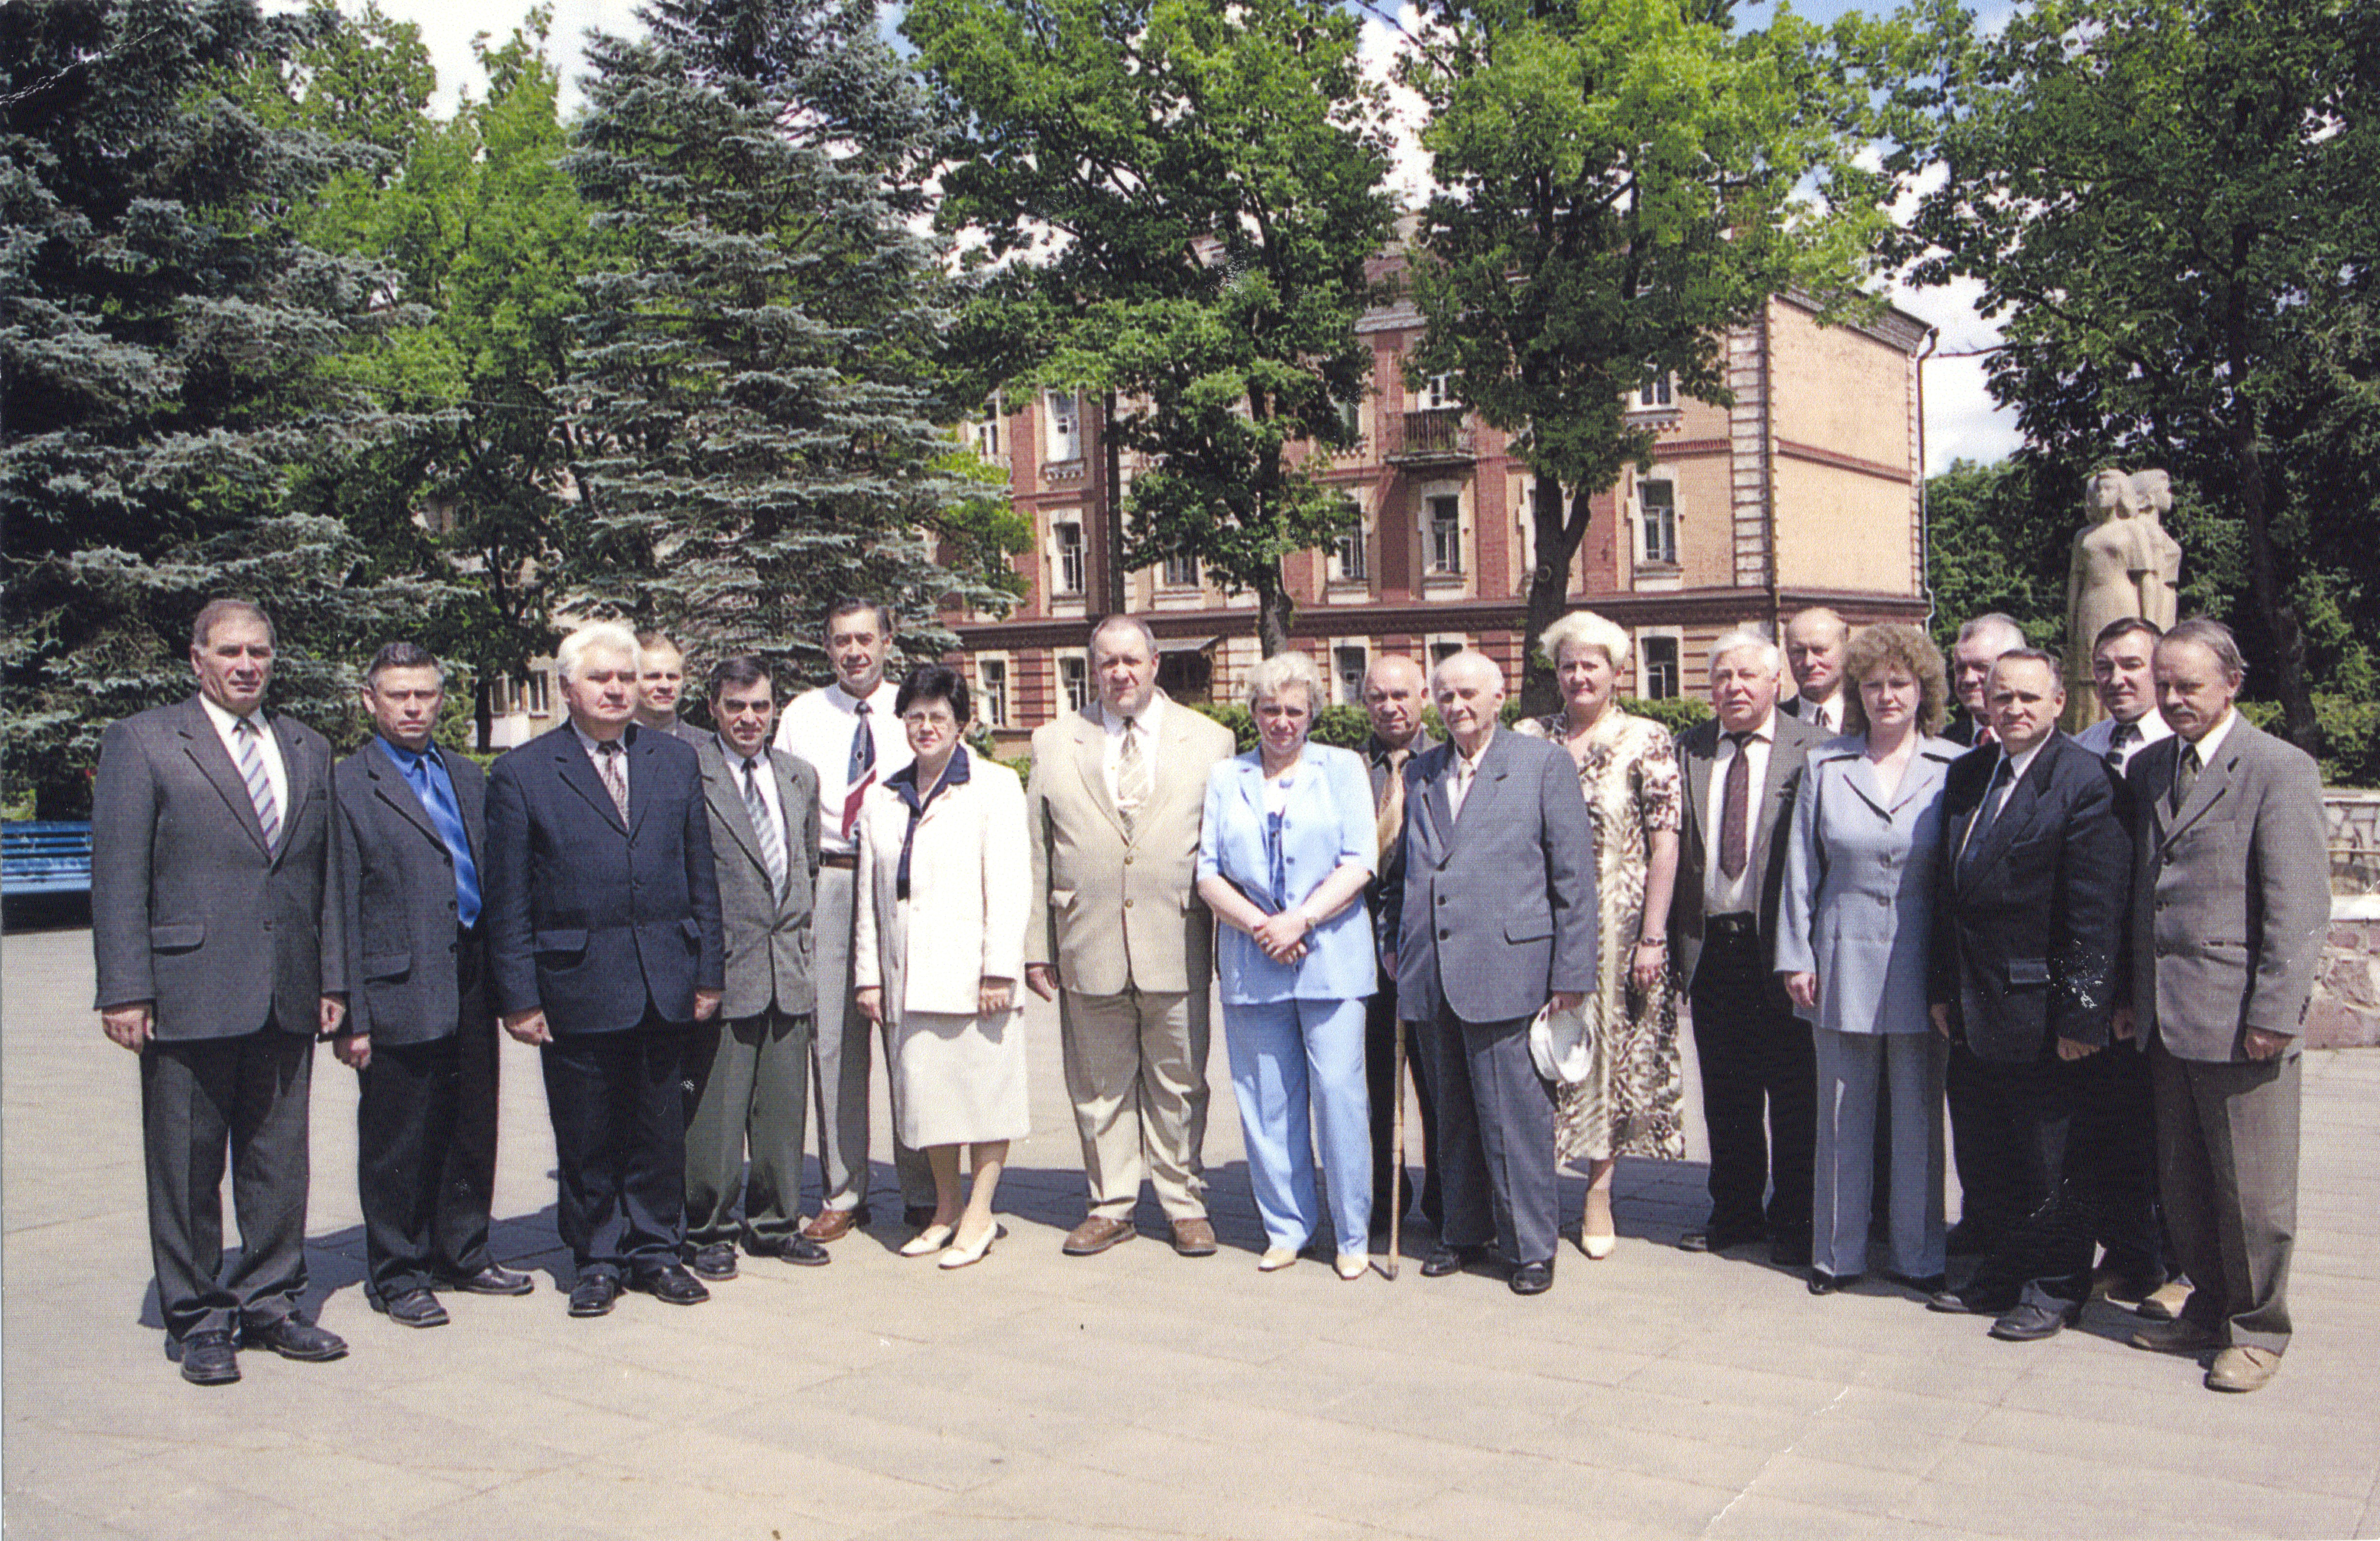
\includegraphics[height=.9\textwidth, width=\textheight, keepaspectratio, angle=90, center]{private/dekaniBsha_attestaciya_2003}
\caption{Эксперты по˚аттестации БСХА и˚деканы факультетов БСХА. М.\,П.~Шубич третий слева. 23\==28.06.2003.}
\label{fig:dekaniBsha_attestaciya_2003}
\end{figure}



\begin{figure}[h]
\includegraphics[height=.9\textwidth, width=\textheight, keepaspectratio, angle=90, center]{private/accreditPenzUniver_2012}
\caption{Аккредитация Пензенского университета архитектуры и˚строительства 19\==23.11.2012. Эксперт Рособрнадзора М.\,П.~Шубич и˚отдельные сотрудники кафедры землеустройства и˚геодезии.}
\label{fig:accreditPenzUniver_2012}
\end{figure}


\begin{figure}[h]
\includegraphics[height=.65\textwidth, width=\textheight, keepaspectratio, angle=90, center]{private/guz_KafedraZeml_2013}
\caption{Кафедра землеустройства ГУЗ. 1\=/ый ряд слева направо: Е.\,В.~Черкашина, В.\,Н.~Сёмочкин, В.\,В.~Пронин, Т.\,А.~Емельянова, С.\,Н.~Волков, В.\,В.~Пименов, М.\,П.~Шубич, Е.\,М.~Чепурин, А.\,В.~Донцов, В.\,В.~Косинский. 2013~год.}
\label{fig:guz_KafedraZeml_2013}
\end{figure}

\todo[Выбор]{Выбрать вариант фото кафедры 1  или 2 }

\begin{figure}[h]
\includegraphics[height=\textwidth, width=\textheight, keepaspectratio, angle=90, center]{private/guz_KafedraZeml_2013_part1}
\caption{Кафедра землеустройства ГУЗ. 1\=/ый ряд слева направо: Е.\,В.~Черкашина, В.\,Н.~Сёмочкин, В.\,В.~Пронин, Т.\,А.~Емельянова, С.\,Н.~Волков. 2013~год. Начало.}
\label{fig:guz_KafedraZeml_2013_part1}
\end{figure}

\begin{figure}[h]
\includegraphics[height=\textwidth, width=\textheight, keepaspectratio, angle=90, center]{private/guz_KafedraZeml_2013_part2}
\caption{Кафедра землеустройства ГУЗ. 1\=/ый ряд слева направо: В.\,В.~Пименов, М.\,П.~Шубич, Е.\,М.~Чепурин, А.\,В.~Донцов, В.\,В.~Косинский. 2013~год. Завершение.}
\label{fig:guz_KafedraZeml_2013_part2}
\end{figure}


\begin{figure}[h]
\includegraphics[height=.9\textwidth, width=\textheight, keepaspectratio, angle=90, center]{private/DelegaciyaChum_2000}
\caption{Делегация у˚чума. М.\,П.~Шубич третий слева. 22.07.2000.}
\label{fig:DelegaciyaChum_2000}
\end{figure}

\begin{figure}[h]
\includegraphics[width=.8\textwidth, center]{private/kater_Solihard_2000}
\caption{На˚катере (Командировка в˚Солихард). М.\,П.~Шубич второй слева. 23.07.2000.}
\label{fig:kater_Solihard_2000}
\end{figure}

\begin{figure}[h]
\includegraphics[width=.8\textwidth, center]{private/ShubichDacha_clip}
\caption{Михаил Павлович Шубич с˚супругой Зинаидой Тихоновной на˚даче.}
\label{fig:ShubichDacha_clip}
\end{figure}


